\chapter{Arquitectura software del sistema}
\label{cap:capitulo6}

\begin{flushright}
\begin{minipage}[]{10cm}
\emph{Un buen desarrollador es aquel que encuentra soluciones a los problemas antes de que surjan}\\
\end{minipage}\\

Bill Gates\\
\end{flushright}

\vspace{1cm}

Una vez definida la arquitectura \textit{hardware} del sistema desarrollado, en este capítulo se presenta la arquitectura \textit{software}, encargada de dar soporte al robot.

\vspace{0.2cm}

La arquitectura se ha diseñado de forma modular con el objetivo de facilitar el desarrollado, mantenimiento, depuración y escalabilidad del sistema. Como se muestra en la (Figura \ref{fig:sistema}), el robot se compone de distintos módulos funcionales. A continuación se procede a definir los distintos módulos software definidos en este proyecto.

\begin{figure} [h!]
  \begin{center}
    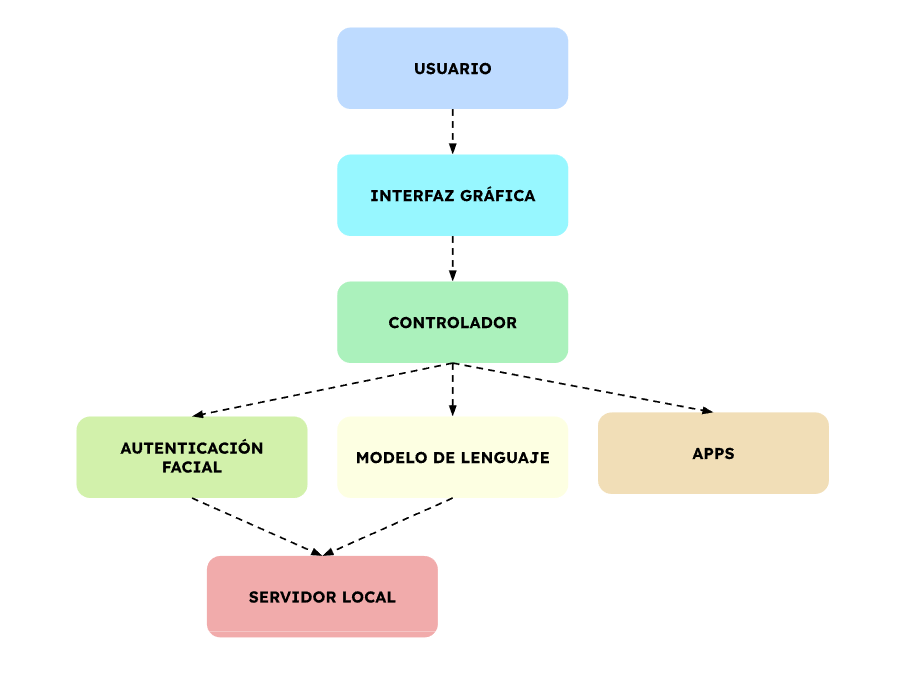
\includegraphics[width=15cm]{figs/sistema}
  \end{center}
  \caption{Servidor local del sistema}
  \label{fig:sistema}
\end{figure}\


\section{Diseño distribuido del sistema}
\label{sec:Sistema de percepción}

Debido a las limitaciones computacionales de la Raspberry Pi 4, no es posible ejecutar tareas de alto coste de computacional. Por ese motivo, se ha diseñado una arquitectura distribuida en la que las tareas más exigentes se delegan a un servidor local.

La arquitectura del sistema se compone de dos elementos principales: la Raspberry Pi 4 integrada en el robot y un ordenador externo que actúa como servidor del sistema.

La Raspberry Pi se encarga de la  gestión de la interfaz gráfica, el control de los periféricos del robot y la coordinación de la interacción con el usuario. Por su parte, el servidor ejecuta los servicios de reconocimiento facial y el modelo de lenguaje conversacional.

La comunicación entre ambos dispositivos se realiza mediante peticiones HTTP a una API que se ha implementado para el sistema, desplegada en una red local privada. Al emplear una red privada se reduce posibles problemas de seguridad.

De este modo, la Raspberry envía solicitudes al servidor para tareas como la identificación del usuario o la generación de respuestas, recibiendo los resultados procesados.

En la (Figura \ref{fig:server}) se muestra la interfaz del servidor local implementado, que permite iniciar los servicios y monitorizar el funcionamiento del sistema en tiempo real.


\vspace{0.2cm}

\begin{figure} [h!]
  \begin{center}
    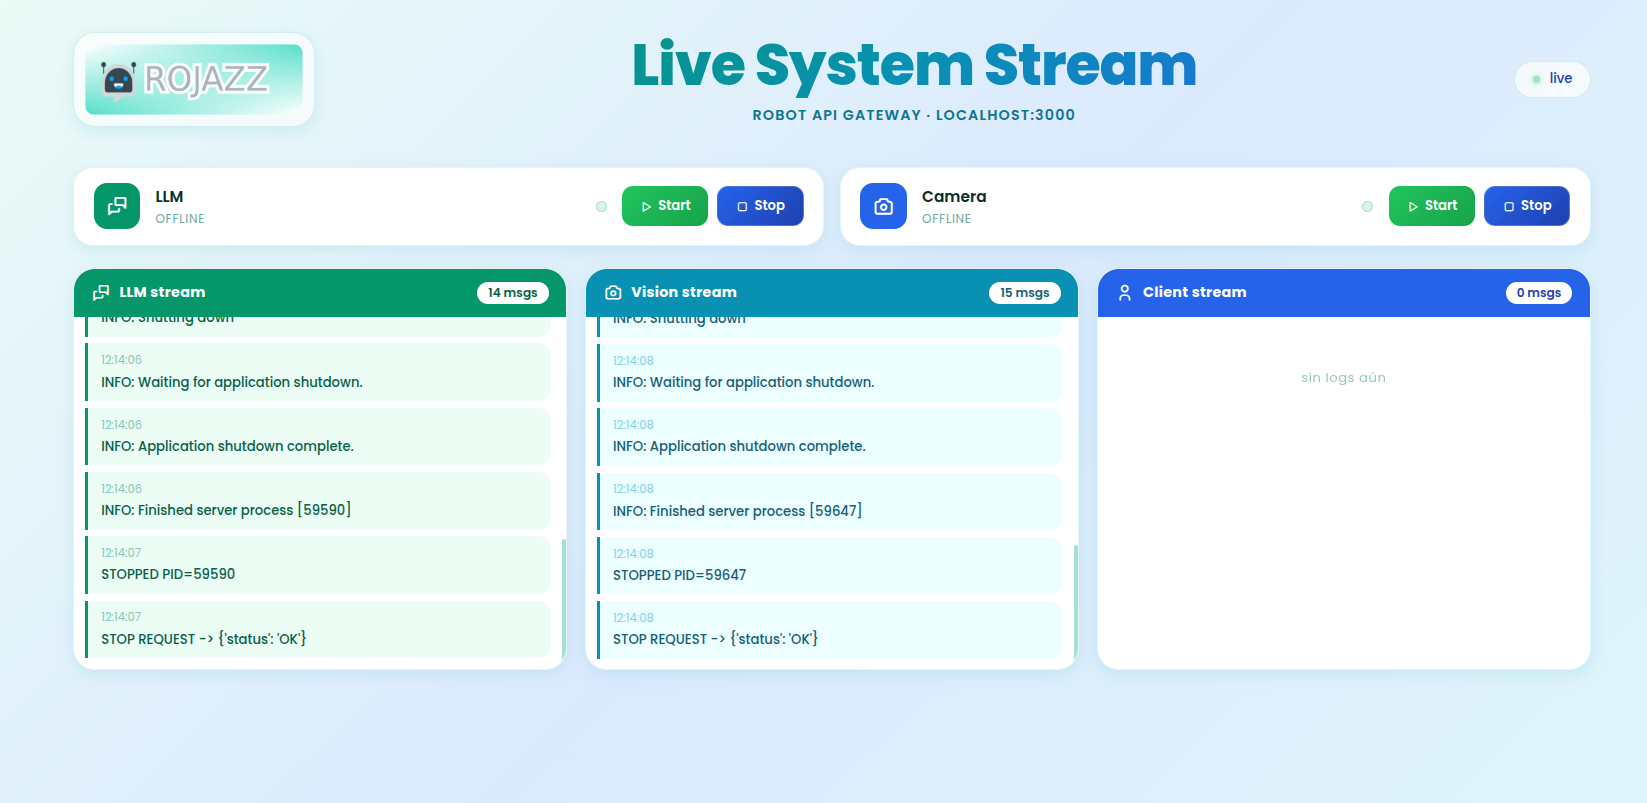
\includegraphics[width=15cm]{figs/server}
  \end{center}
  \caption{Servidor local del sistema}
  \label{fig:server}
\end{figure}\


\section{Redes y comunicaciones}
\label{sec:Sistema de percepción}

Para asegurar una comunicación estable entre la Raspberry Pi y el servidor, se ha utilizado un router propio configurado con una red local privada. De este modo, ambos dispositivos poseen direcciones IP fijas, evitando problemas cambios de direccione IP.


\section{Sistema de autenticación facial}
\label{sec:Sistema de percepción}

El sistema de autenticación facial compone el paso inicial para el arranque del sistema de asistencia personal. Este módulo se apoya en la arquitectura distribuida previamente descrita.

\vspace{0.2cm}

El sistema se divide en dos fases principales: registro de usuarios e inicio de sesión.

\vspace{0.2cm}

Durante la fase de registro, la Raspberry Pi captura varias imágenes del usuario a través de la cámara integrada en el robot. Estas imágenes se envían al servidor mediante peticiones HTTP, donde se realiza la detección facial y la extracción de características mediante vectores de representación (\textit{face embeddings}) utilizando la librería \verb|face_recognition|.

Los \textit{embeddings} generados se almacenan junto con la etiqueta del usuario un fichero \texttt{.pkl}, el cual permite la incorporación  de nuevos usuarios en el sistema de forma persistente.

\vspace{0.2cm}


En la fase de inicio de sesión, el sistema captura imágenes en tiempo real y las envía al servidor. Este calcula los \textit{embeddings} y las compara con los almacenadas en la base de datos de rostros conocidos, como se puede ver en el Código \ref{cod:codejemplo}. El reconocimiento facial se realiza mediante la distancia entre vectores, seleccionado el usuario más similar en el caso de superar el umbral de parecido establecido.


\begin{code}[h]
\begin{lstlisting}[language=python]

locations = face_recognition.face_locations(rgb)
encodings = face_recognition.face_encodings(rgb, locations)

print(f"[RECOGNIZE] Cara encontrada: {len(encodings)}", flush=True)

results = []

for enc in encodings:
    matches = face_recognition.compare_faces(known_face_encodings, enc)
    name = "Desconocido"

    if len(matches) > 0:
        dists = face_recognition.face_distance(known_face_encodings, enc)
        best = np.argmin(dists)
        if matches[best]:
            name = known_face_names[best]

    results.append(name)

print(f"[RECOGNIZE] resultado: {results}", flush=True)
return {"recognized": results}

\end{lstlisting}
\caption[Función para detección y reconocimiento facial]{Función para detección y reconocimiento facial}
\label{cod:codejemplo}
\end{code}

Este sistema de autenticación permite el acceso al resto de funcionalidades del robot de forma personalizada.


\section{Sistema conversacional}
\label{sec:Sistema conversacional}

El sistema conversacional constituye el núcleo de interacción entre el usuario y el robot, permitiendo la comunicación mediante lenguaje natural. Este módulo se apoya en la arquitectura distribuida anteriormente descrita.

\vspace{0.2cm}

La arquitectura del sistema conversacional está compuesta por una serie de etapas consecutivas: captura de audio, transcripción del audio, procesamiento mediante un modelo de lenguaje natural, y conversión del texto generado a voz.

El sistema permanece en un estado de escucha continua y únicamente se activa cuando se detecta una palabra de activación predefinida. Este mecanismo evita respuestas no deseadas y agotar recursos del sistema.

\subsection{Captura de audio y transcripción del habla}

Mediante el uso del micrófono integrado en el robot se captura el audio del usuario. El sistema utiliza el motor de reconocimiento de voz \textit{vosk}, que permite transcribir en tiempo real de forma local, asegurando así la privacidad del usuario.

\vspace{0.2cm}

El flujo de escucha se implementa como un proceso continuo, en el que se analiza el audio en busca de la palabra de activación. Una vez detectada, el sistema conversacional se activa, habilitando la interacción con el usuario, como se muestra en el Código \ref{cod:wake_word}.

\begin{code}[h]
\begin{lstlisting}[language=python]
# Fragmento simplificado del sistema de escucha
if self.wake_word in text.lower():
    self.active = True
    print("WAKE ACTIVATED")
\end{lstlisting}
\caption{Detección de palabra de activación en el sistema de reconocimiento de voz}
\label{cod:wake_word}
\end{code}


\subsection{Procesamiento del lenguaje natural}

Una vez transcrito el mensaje, el texto resultante se envía mediante una petición HTTP al servidor. Este servidor se encarga del procesamiento del lenguaje natural utilizando modelos de lenguaje, en este caso \textit{Llama 3.3}. El servidor recibe la petición, genera una respuesta y la devuelve a la Raspberry.

En el Código \ref{cod:codejemplo3} se muestra la estructura del endpoint encargado de generar las respuestas.


\begin{code}[h]
\begin{lstlisting}[language=python]
@app.post("/generate")
def generate(payload: dict):
    model_name = payload.get("model")
    prompt = payload.get("prompt")
    output = model.generate(prompt)
    return {"output": output}
\end{lstlisting}
\caption{Endpoint de generación de respuestas del modelo de lenguaje}
\label{cod:codejemplo3}
\end{code}


\subsection{Síntesis de voz}
\vspace{0.2cm}

Una vez generada la respuesta, esta se envía a la Raspberry Pi, donde se convierte en audio mediante el uso de \textit{pico2wave}, una herramienta de software libre que convierte texto a voz.

\vspace{0.2cm}

El módulo de síntesis incluye un proceso de limpieza del texto para aportar mayor naturalidad a la voz generada, eliminando caracteres especiales y estructuras no necesarias.



\section{Interfaz gráfica}
\label{sec:Interfaz gráfica}

Para permitir la interacción del usuario con las diferentes funcionalidades del robot, se ha desarrollado una interfaz gráfica encargada de proporcionar acceso a los distintos módulos del sistema.

\vspace{0.2cm}

La interfaz se ha implementado utilizando la biblioteca \verb|PyQt5| y se ejecuta en la Raspberry Pi. El diseño se ha basado en una arquitectura basada en estados, donde cada pantalla representa una funcionalidad distinta del sistema. La transición entre pantallas se realiza mediante eventos gestionados por un controlador central.

\vspace{0.2cm}

La interfaz se muestra en una pantalla táctil integrada en el robot. Adicionalmente, el sistema incorpora una pantalla LCD destinada a mostrar información sobre el estado del robot.

\vspace{0.2cm}

Las principales pantallas desarrolladas son:

\begin{itemize}
    \item Pantalla de autenticación facial.
    \item \textit{Launcher} principal de aplicaciones.
    \item Aplicaciones internas (notas, calendario, recordatorios, juegos, etc.).
\end{itemize}


El \textit{launcher} actúa como núcleo de navegación del sistema, permitiendo acceder a las funcionalidades del sistema.

\vspace{0.2cm}

La pantalla de autenticación constituye el punto de entrada del sistema y permite identificar o registrar un usuario. Una vez autenticado, este accede automáticamente al \textit{launcher}, que proporciona acceso al resto de aplicaciones disponibles.

\vspace{0.2cm}

Durante el diseño de la interfaz se ha priorizado la accesibilidad, teniendo en cuenta que el sistema está orientado a personas mayores. Para ello se optado por la utilización de botones de gran tamaño, iconografía fácilmente reconocible y una navegación sencilla.

Las (Figuras \ref{fig:login} y \ref{fig:launcher}) muestran las principales pantallas implementadas para la interacción con el usuario.


\vspace{0.2cm}

\begin{figure} [h!]
  \begin{center}
    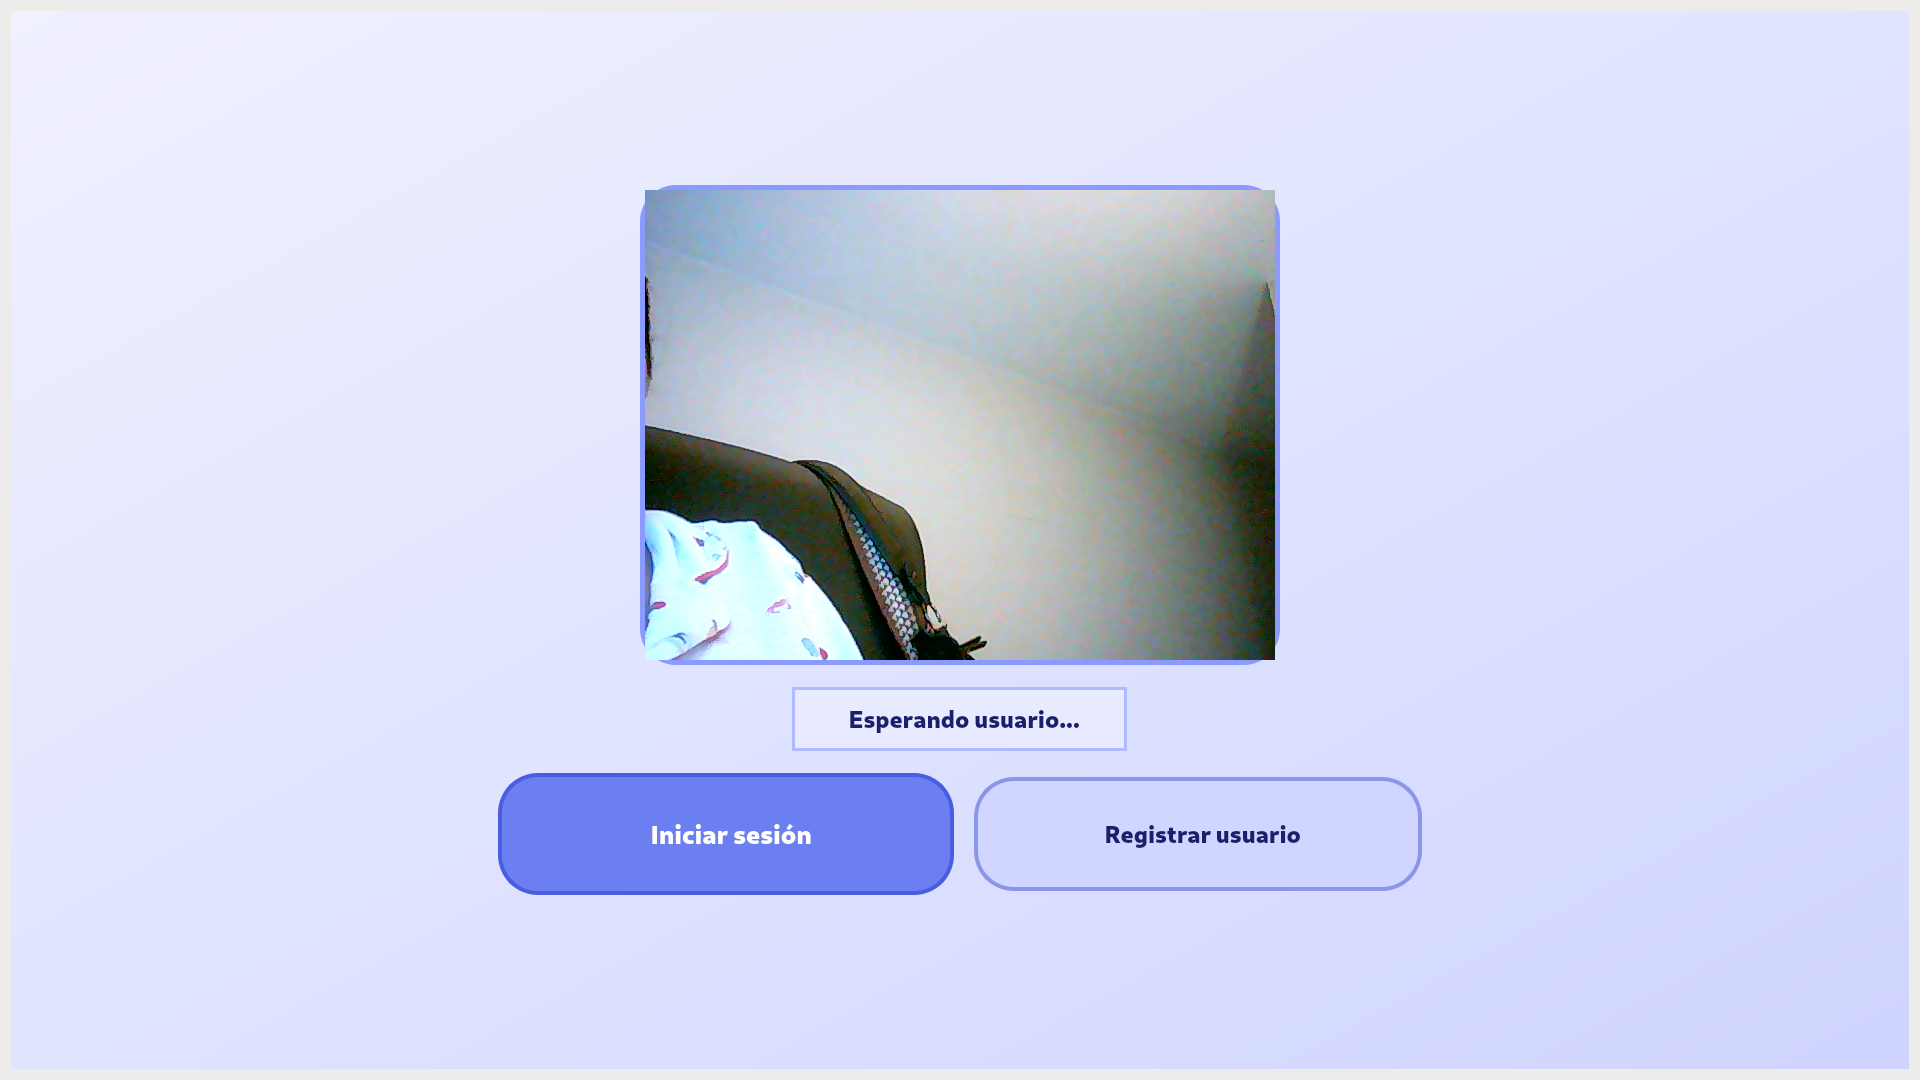
\includegraphics[width=15cm]{figs/login}
  \end{center}
  \caption{Pantalla del \textit{login}}
  \label{fig:login}
\end{figure}\


\begin{figure} [h!]
  \begin{center}
    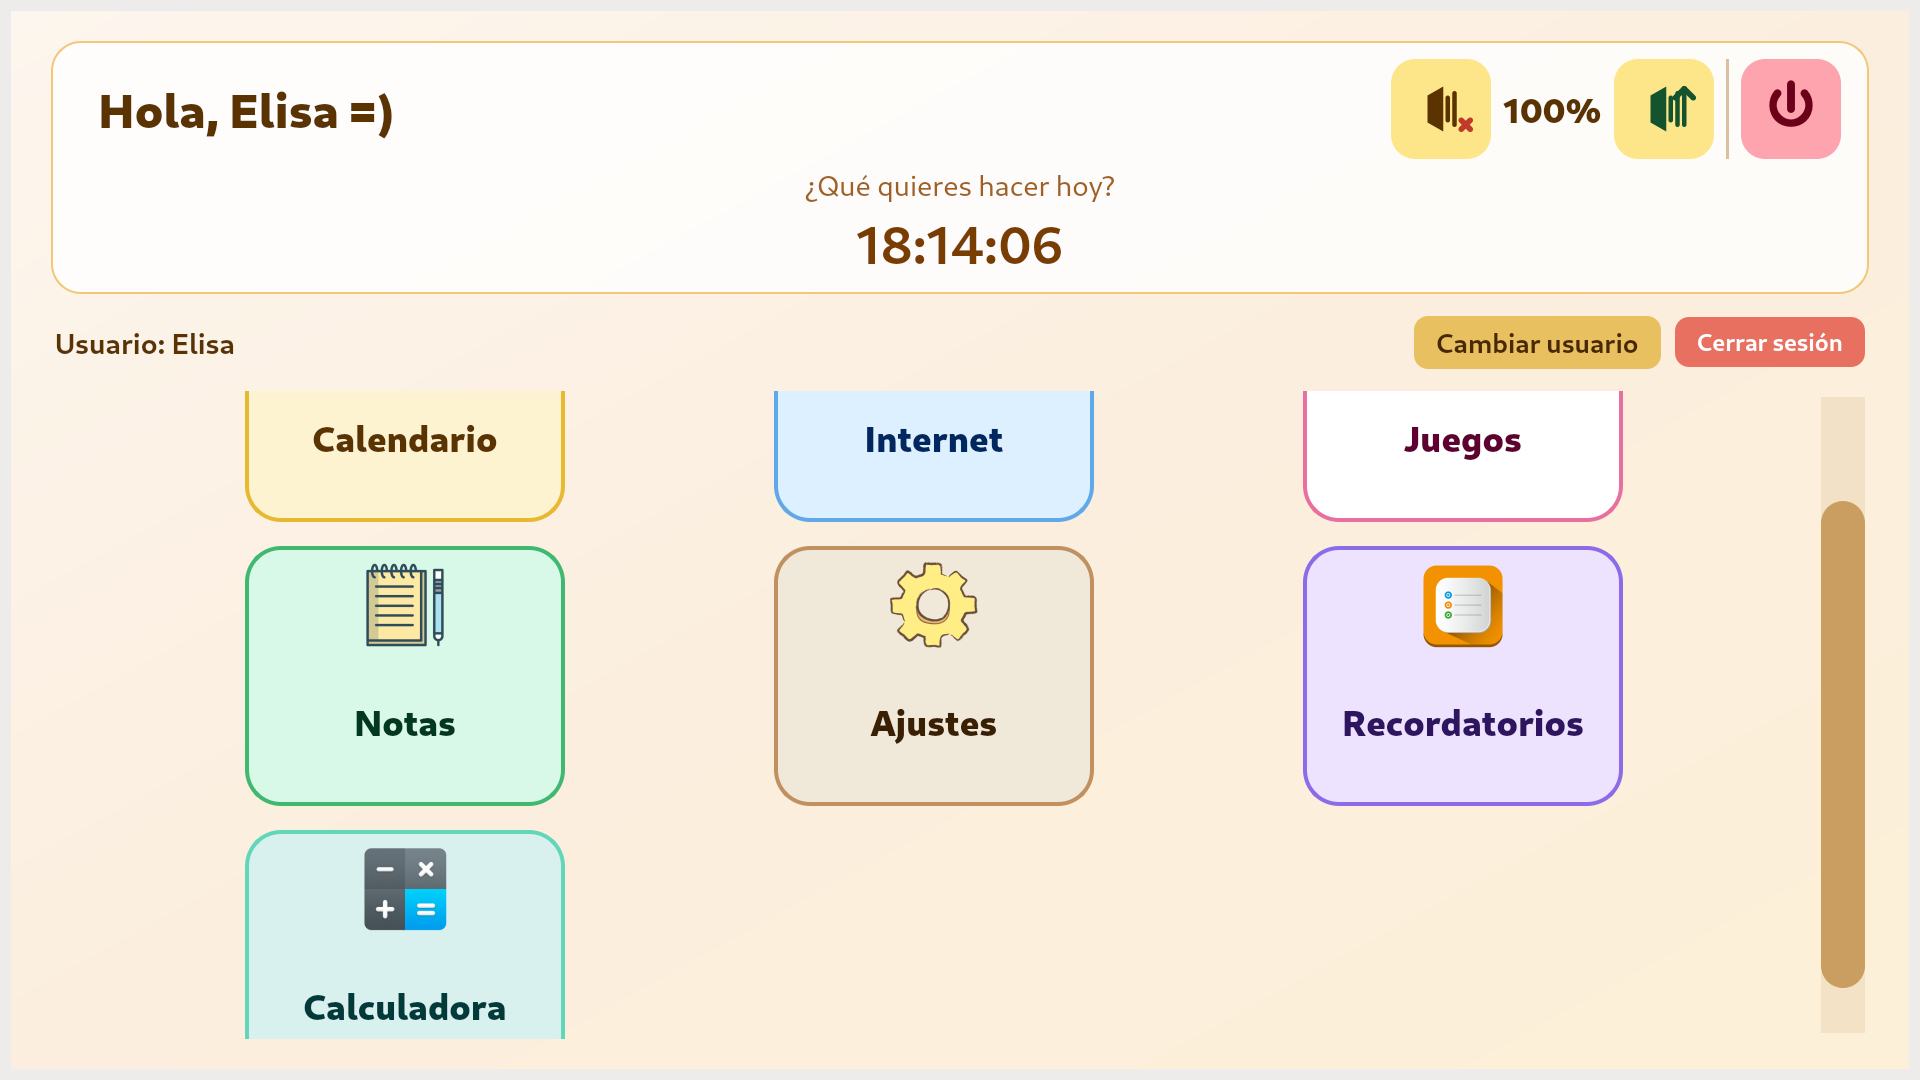
\includegraphics[width=15cm]{figs/launcher}
  \end{center}
  \caption{Pantalla del \textit{launcher}}
  \label{fig:launcher}
\end{figure}\



\section{Controlador central}
\label{sec:Controlador central}

El controlador se comporta como un intermediario entre los distintos módulos del sistema.
Su principal tarea consiste en gestionar el flujo de ejecución mediante un modelo basado en estados, asegurando que cada componente se active en el momento adecuado.

\vspace{0.2cm}

Tal como se muestra en el Código \ref{cod:controller}, el controlador se encarga de inicializar los principales módulos del sistema, incluyendo el gestor de sesión de usuarios, el motor de asistente y el sistema de la visualización de estado del robot.


\begin{code}[h]
\begin{lstlisting}[language=python]
self.state_machine = StateMachine()
self.session = SessionManager()

self.display = FaceDisplay()
self.display.start()

self.assistant = AssistantEngine(
    ui_state=self.ui_state,
    face_display=self.display
)
\end{lstlisting}
\caption{Inicialización de componentes en el controlador central}
\label{cod:controller}
\end{code}


El controlador gestiona el arranque del sistema, el proceso de autenticación del usuario, el acceso al \textit{launcher} y el cierre controlado del robot.

\vspace{0.2cm}

Una vez autenticado el usuario, el controlador actualiza el estado del sistema y habilita el asistente conversacional. Del mismo modo, mantiene sincronizados el estado interno del sistema y la interfaz gráfica, coordinando la apertura y cierre de las aplicaciones.


Este diseño modular facilita el mantenimiento del sistema, mejora su escalabilidad y permite la incorporación de nuevas funcionalidades sin afectar al sistema general.


\section{Sistema de asistencia proactiva}
\label{sec:Sistema de asistencia proactiva}

Además de la interacción mediante interfaz gráfica y comunicación por voz, el sistema incorpora un módulo de asistencia proactiva que tiene como objetivo fomentar la actividad del usuario.

\vspace{0.2cm}

Este módulo se encarga de generar sugerencias de forma periódica y autónoma. Dichas recomendaciones incluyen actividades físicas ligeras, así como la interacción con algunas aplicaciones disponibles.

El comportamiento de este sistema se basa en eventos programados. Cuando se detecta que ha trascurrido un período de tiempo definido, el sistema genera una sugerencia de forma aleatoria, la cual se presenta en la interfaz gráfica y mediante síntesis de voz.

En la siguiente (Figura \ref{fig:sugerencia}) se muestra un ejemplo de las sugerencias generadas por este módulo.

\begin{figure} [h!]
  \begin{center}
    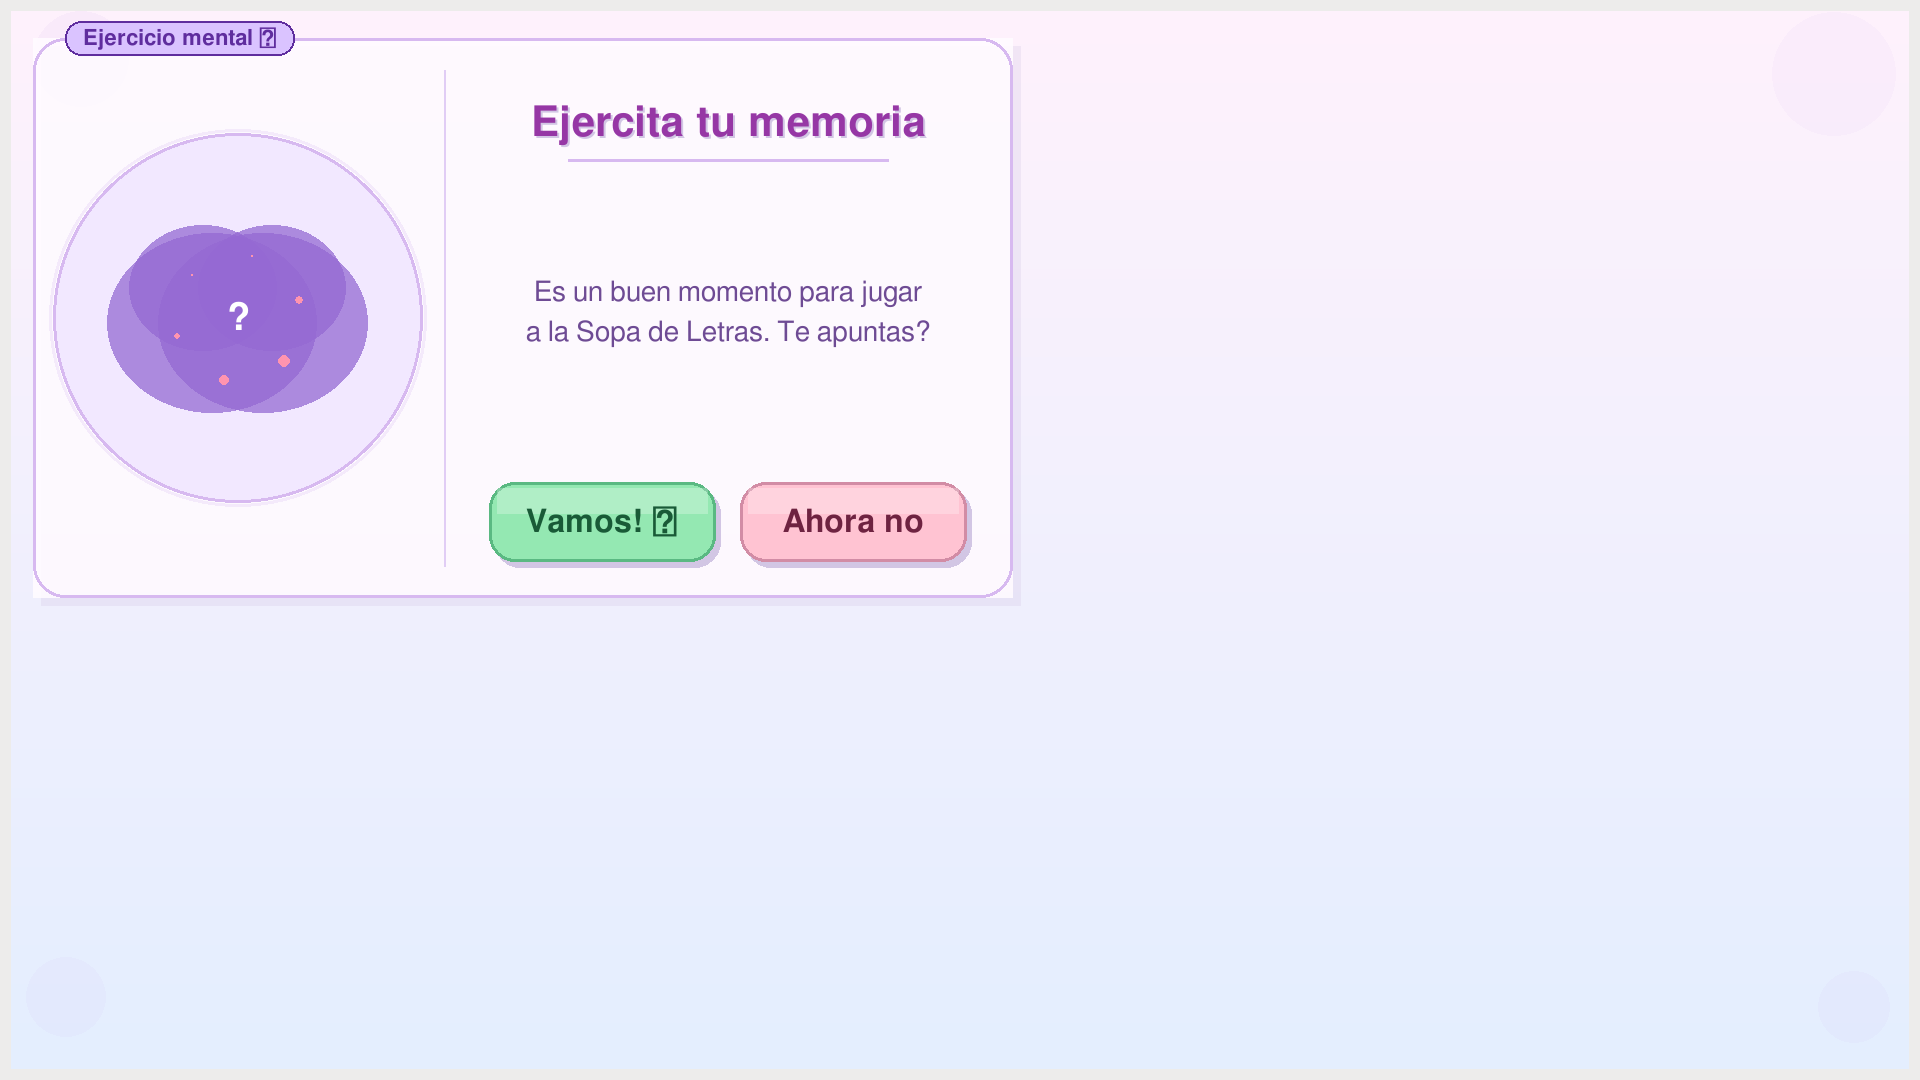
\includegraphics[width=15cm]{figs/sugerencia}
  \end{center}
  \caption{Pantalla de sugerencia generada por el sistema de asistencia proactiva}
  \label{fig:sugerencia}
\end{figure}\



\section{Aplicaciones desarrolladas}
\label{sec:Aplicaciones desarrolladas}

El sistema incluye una serie de aplicaciones internas diseñadas para evitar que la interacción con el robot se limite únicamente a la recepción de respuestas. Estas aplicaciones se gestionan mediante el controlador central, lo que permite mantener un coherente del sistema en todo momento.

\vspace{0.2cm}

Entre las aplicaciones desarrolladas se incluyen el calendario, el sistema de recordatorios, el gestor de notas y un conjunto de juegos orientados el entrenamiento cognitivo. Todas las aplicaciones están desarrolladas sobre \textit{PyQt5} y se integran dentro del flujo de navegación gestionado por el \textit{launcher} principal.
La aplicación de calendario (Figura \ref{fig:calen}) permite gestionar de forma visual los eventos del usuario y garantizando la persistencia de los datos entre sesiones.

\begin{figure} [h!]
  \begin{center}
    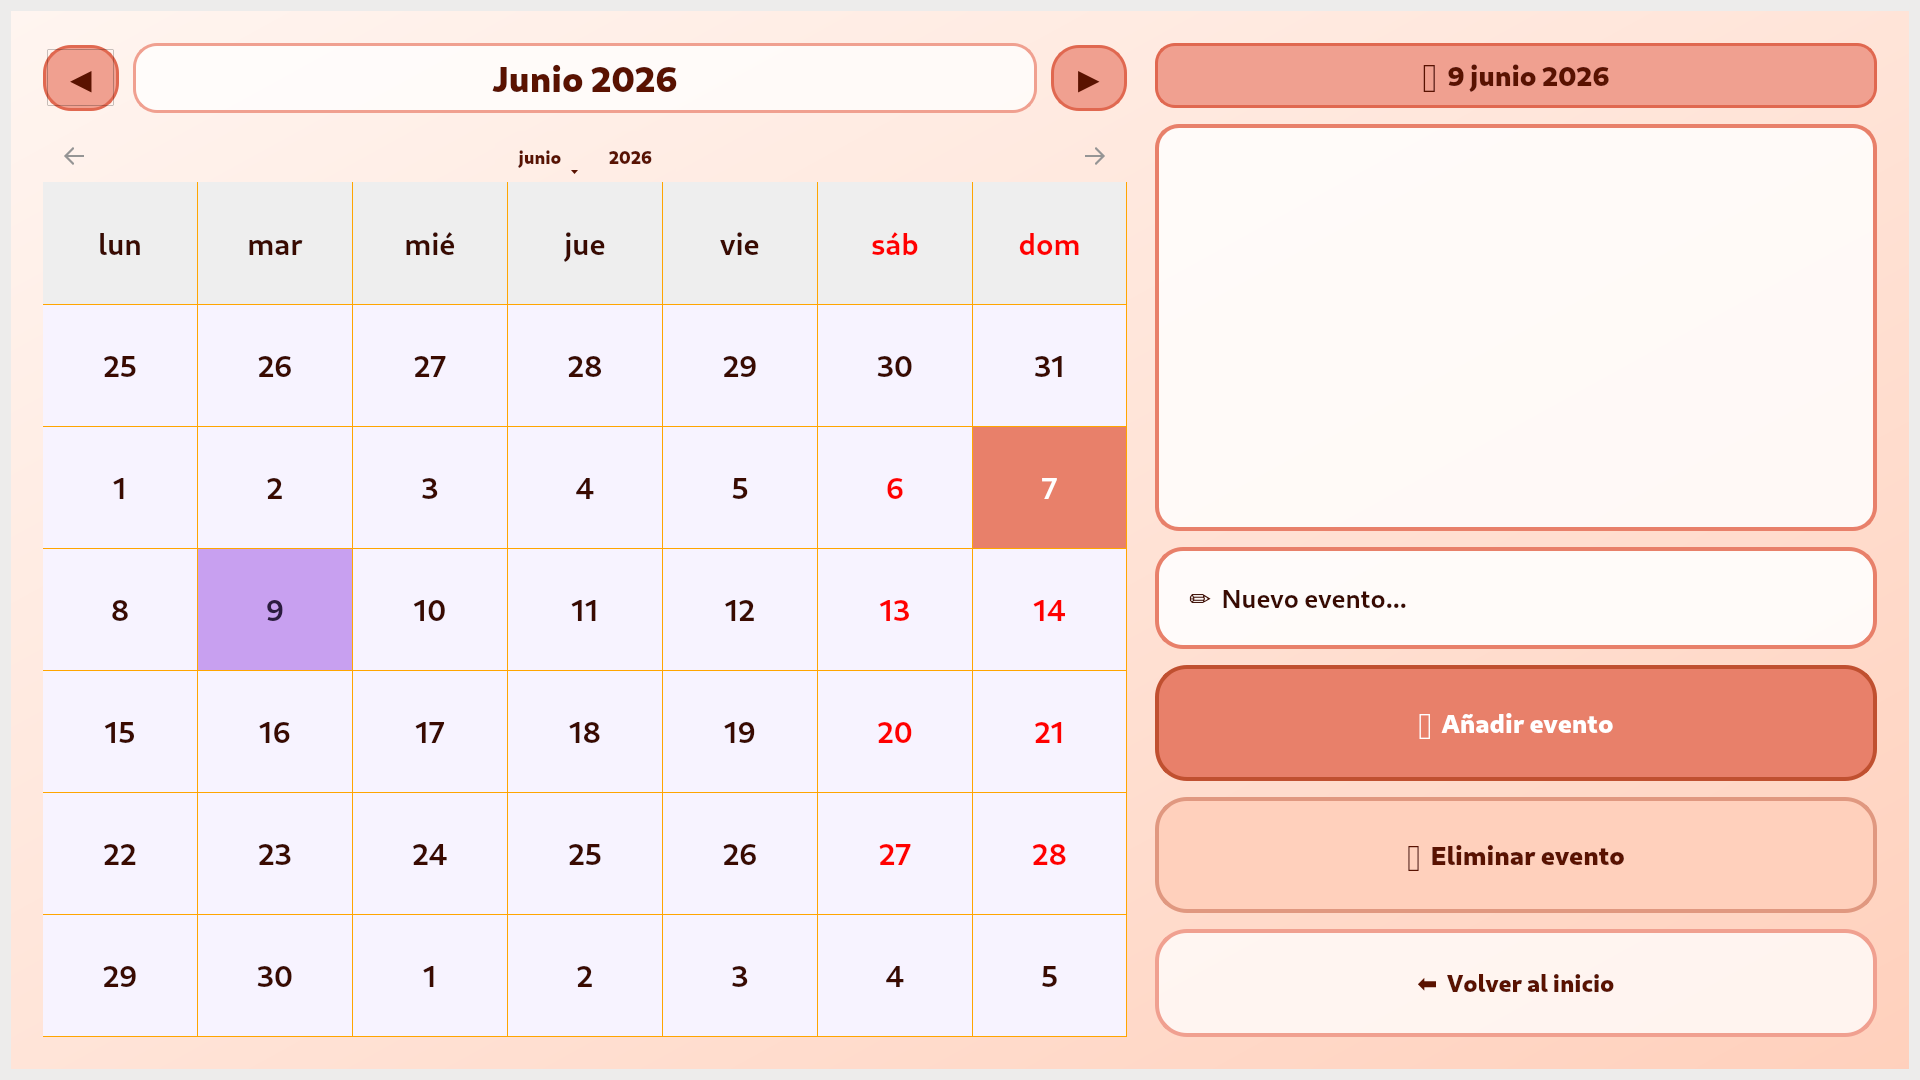
\includegraphics[width=15cm]{figs/calen}
  \end{center}
  \caption{Pantalla del calendario}
  \label{fig:calen}
\end{figure}\

La interacción con esta aplicación permite la creación, eliminación y visualización de eventos de forma intuitiva.

\vspace{0.2cm}

Por otro lado, el sistema de recordatorios permite al usuario gestionar avisos pendientes. Esta funcionalidad (Figura \ref{fig:rec}) sigue una estructura similar a la aplicación de calendario, compartiendo modelo de persistencia y visualización.

\begin{figure} [h!]
  \begin{center}
    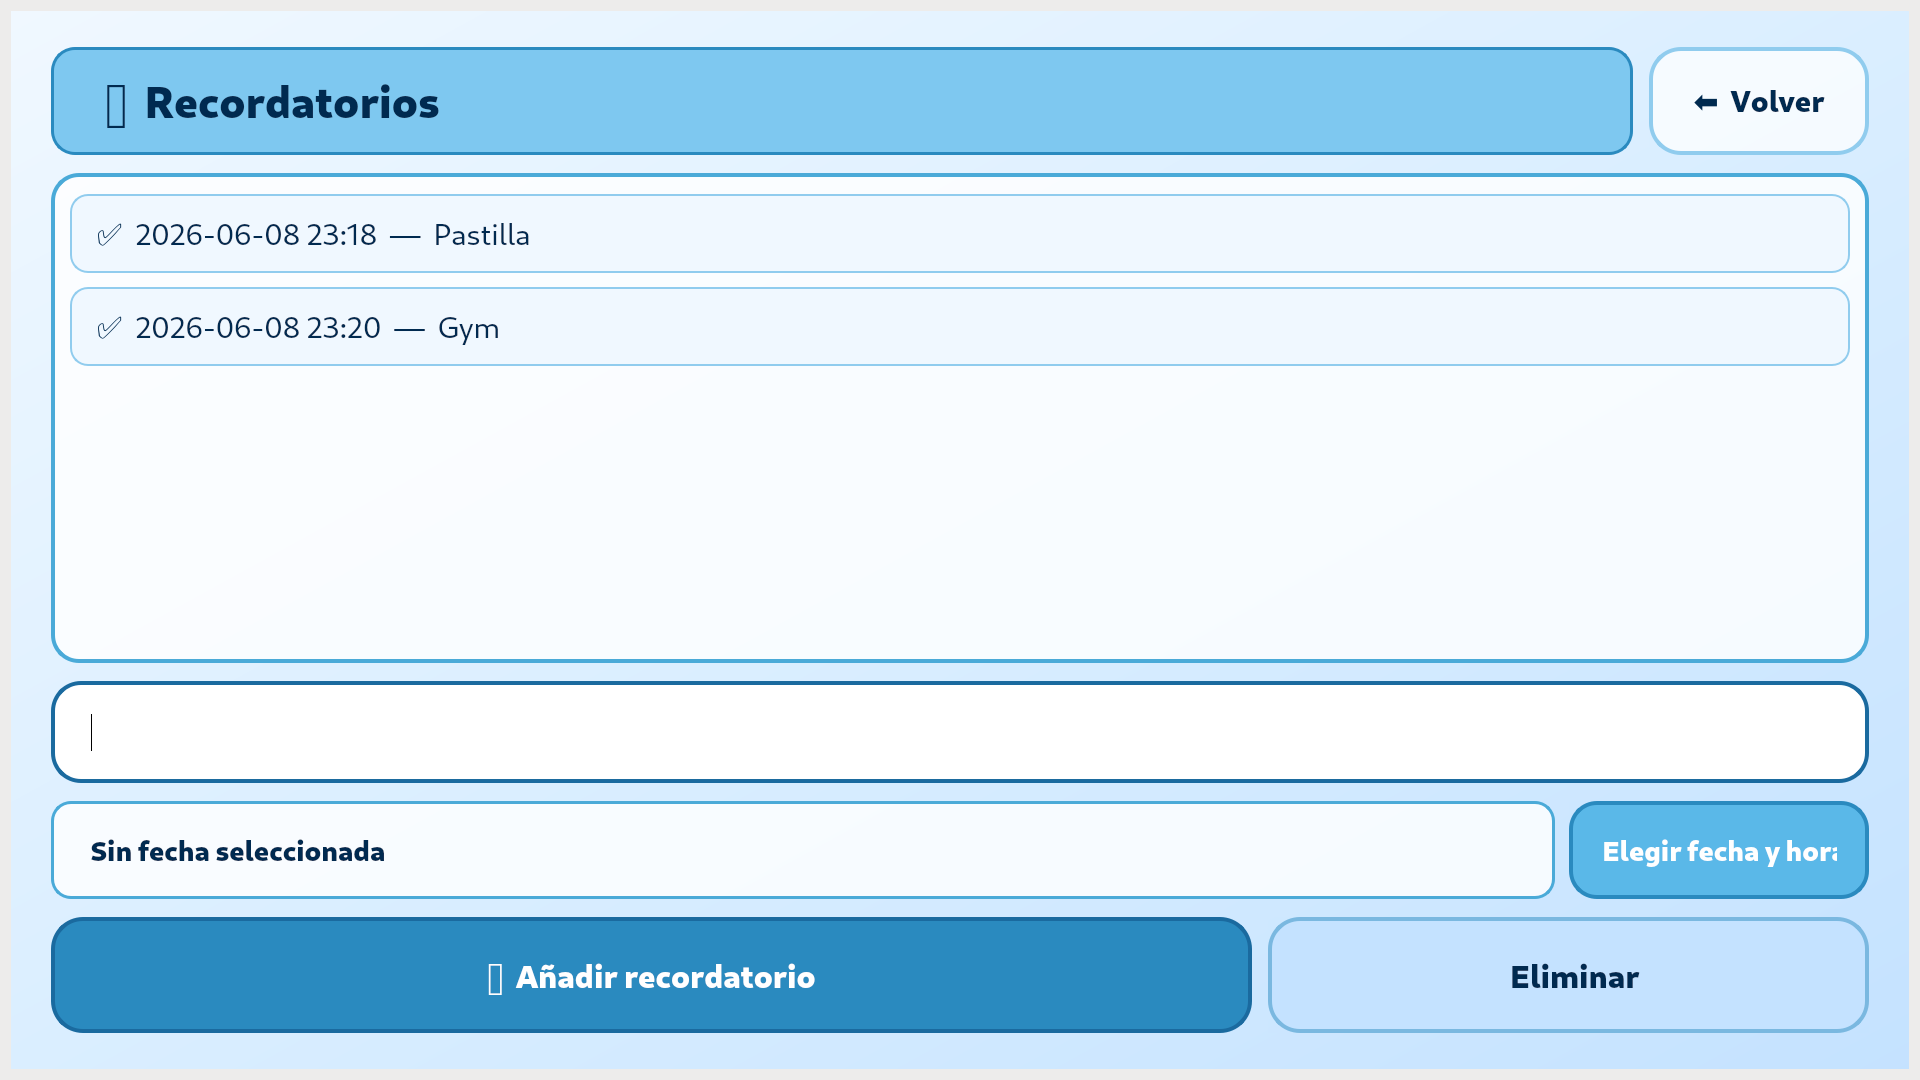
\includegraphics[width=15cm]{figs/rec}
  \end{center}
  \caption{Pantalla de recordatorios}
  \label{fig:rec}
\end{figure}\


Además de la interacción táctil, estas aplicaciones pueden ser controladas mediante comandos de voz. El sistema conversacional es capaz de interpretar intenciones relacionadas con la gestión de las distintas funcionalidades, permitiendo al usuario crear eventos o recordatorios mediante expresiones naturales como: ``añade una cita mañana a las diez'' o ``recuérdame comprar medicación''.

\vspace{0.2cm}

Cuando se detecta una intención de este tipo, el sistema llama a la aplicación mediante el controlador, que actúa como intermediario entre el módulo conversacional y las aplicaciones.

\vspace{0.2cm}

El diseño de las aplicaciones sigue un enfoque sencillo y accesible, utilizando una paleta de colores suaves y elementos de gran tamaño para facilitar su uso.

\vspace{0.2cm}

En las aplicaciones con campos de texto se incorpora un teclado virtual que se activa dinámicamente cuando el usuario interactúa con campos de texto, sin necesidad de periféricos externos.

\vspace{0.2cm}


Adicionalmente, el sistema cuenta con un conjunto de juegos orientados a fomentar la actividad cognitiva del usuario. Se incluyen actividades como sopa de letras, \textit{Simon Says}, juego de memoria y búsqueda de diferencias.

Estos juegos ayudan a mantener capacidades cognitivas básicas como memoria visual, agilidad mental o atención, resultando de gran utilidad en el contexto de usuarios de edad avanzada.

Estos juegos siguen el mismo enfoque sencillo que el resto de aplicaciones del sistema, con elementos visuales de gran tamaño y una interacción intuitiva.

En la (Figura \ref{fig:mem}) se muestra el juego de memoria desarrollado.

\vspace{0.2cm}

\begin{figure}[h!]
  \centering
  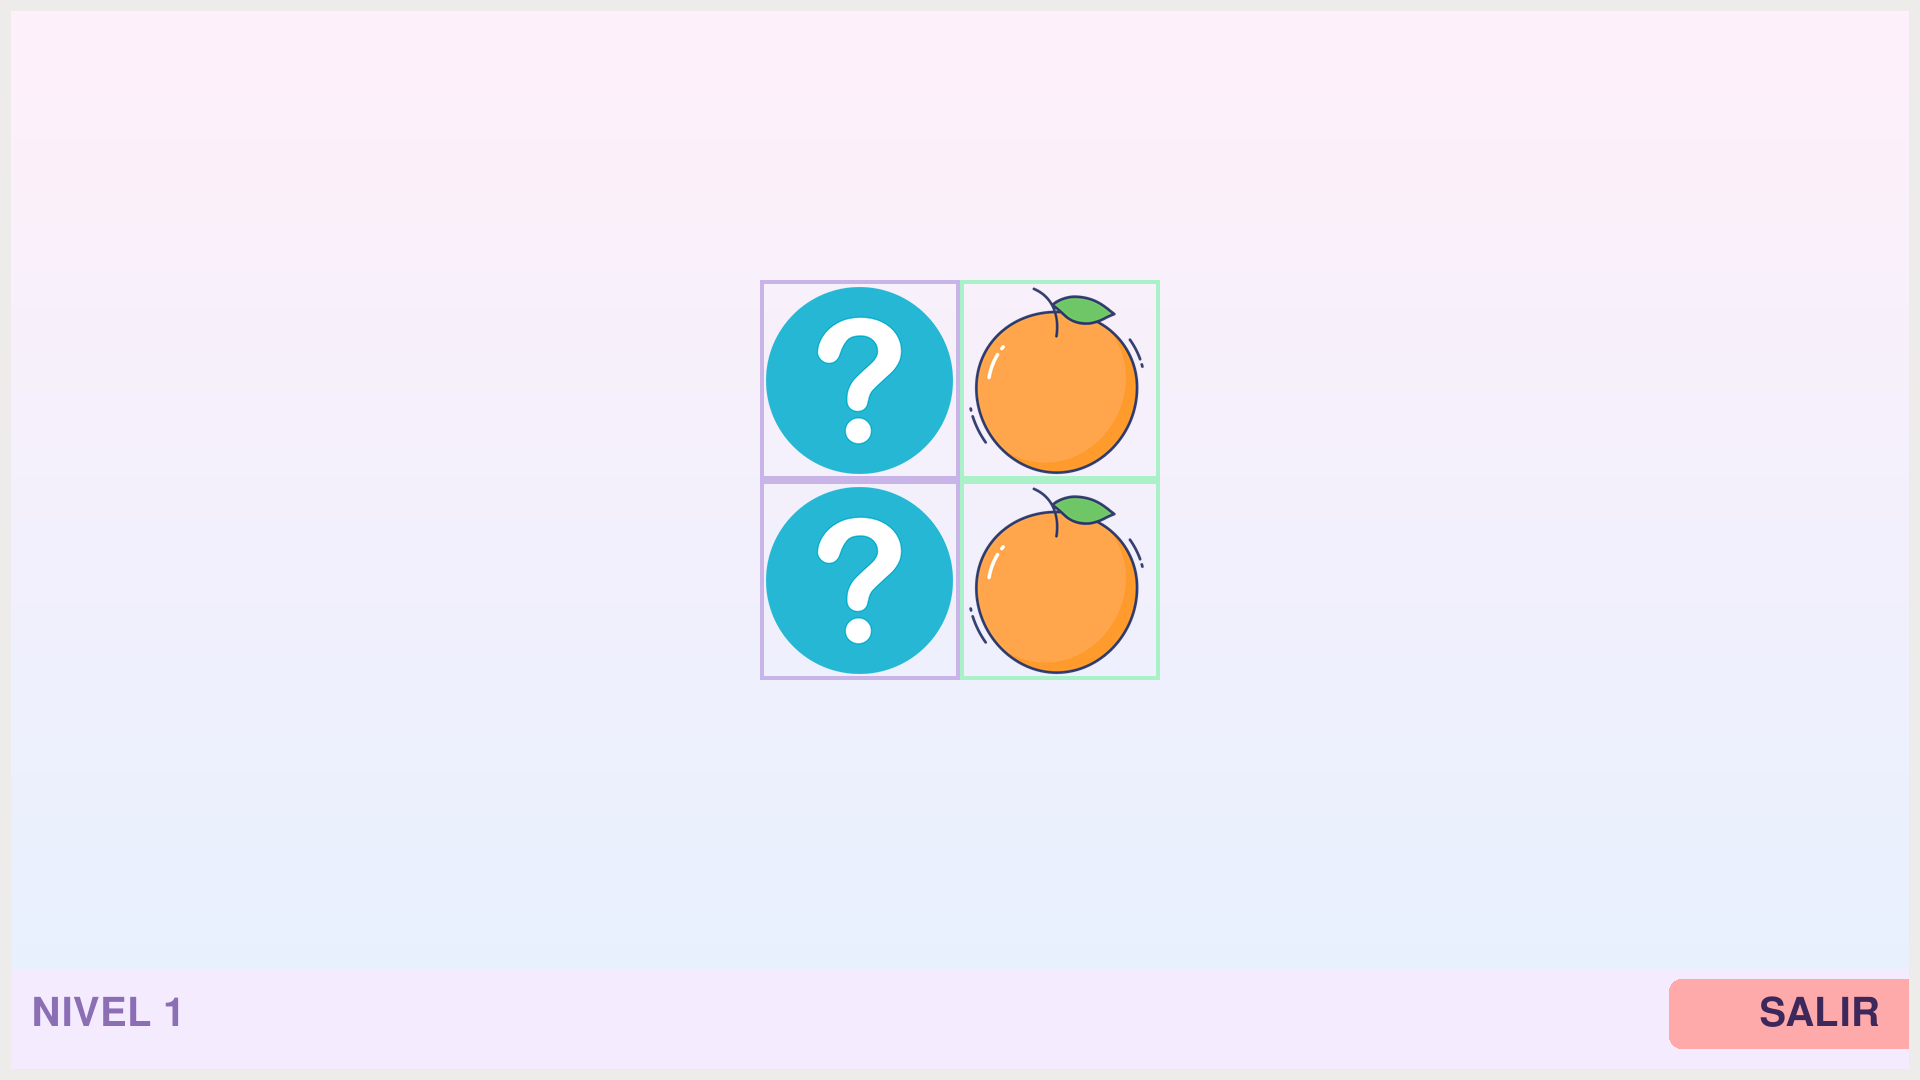
\includegraphics[width=0.95\textwidth]{figs/mem}
  \caption{Interfaz del sistema de juegos de estimulación cognitiva}
  \label{fig:mem}
\end{figure}

